\documentclass{ximera}

\newcommand{\RR}{\mathbb R}
\renewcommand{\d}{\,d}
\newcommand{\dd}[2][]{\frac{d #1}{d #2}}
\renewcommand{\l}{\ell}
\newcommand{\ddx}{\frac{d}{dx}}
\newcommand{\dfn}{\textbf}
\newcommand{\eval}[1]{\bigg[ #1 \bigg]}

\author{Jim Talamo}
\outcome{Use the divergence test to determine that a series diverges.}
\outcome{Understand why the terms in a convergent series must tend to zero.}
\outcome{Answer conceptual questions that utilize both the definition of convergence and the divergence test.}
\outcome{Recognize known convergent or divergent series.}

\title[Dig-In:]{The divergence test}

\begin{document}
\begin{abstract}
If an infinite sum converges, then its terms must tend to zero.
\end{abstract}
\maketitle

In order to determine if a \emph{series} $\sum_{k=1}^{\infty} a_k$ converges, we took the following approach.

\begin{itemize}
\item[1.] Consider the associated sequence $\{s_n\}$ of partial sums, where $s_n=\sum_{k=1}^n a_k$.
\item[2.] Try to find an explicit formula for the term $s_n$.  If you can find such a formula, analyze $\lim_{n \to \infty s_n}$.  
\begin{itemize}
\item If the limit exists, $\sum_{k=k_0} a_k$ converges, and if we can determine that $\lim_{n \to \infty} s_n =L$, then $\sum_{k=k_0} a_k=L$.  \item If  $\lim_{n \to \infty} s_n$ does not exist, then $\sum_{k=k_0} a_k$ diverges.
\end{itemize}
\item[3.] If an explicit formula for $s_n$ cannot be found, further analysis is needed.  
\end{itemize}

In the previous section, we studied two types of series where we could find an explicit formula for $s_n$, but unfortunately, this is not always easy or possible.  Fortunately, it is not always necessary to do this in order to determine whether $\lim_{n \to \infty} s_n$ exists.  Consider the example below.

\begin{example}
Determine if the series $\sum_{k=1}^{\infty} \frac{k+2}{2k+1}$ converges or diverges.  

\begin{explanation}
Let's think about what we are trying to do here heuristically.  If we set $a_k =  \frac{k+2}{2k+1}$, we can write out the first several terms in the sequence $\{a_n\}_{n=1}$.

\[
\frac{3}{5}, \frac{4}{7}, \frac{5}{9}, \frac{6}{11},\frac{7}{13}, \ldots
\]
We can observe also that $\lim_{n \to \infty} a_n = \answer[given]{\frac{1}{2}}$, so eventually, the terms in this list become as close to $\frac{1}{2}$ as we want.  Conceptually, we can interpret that when trying to compute the series, we will have to add infinitely many numbers together that are very close to $\frac{1}{2}$.  Such an attempt cannot produce a finite result, so we expect the series to diverge.

Of course, this is not a formal proof or an acceptable mathematical argument, but it is good intuition.  In order to formalize the argument, recall that we have to set $s_n = \sum_{k=1}^n a_k$ and study whether $\lim_{n \to \infty} s_n$ exists.  While we do not have an explicit formula for $s_n$, we do have a recursive formula, which we recall below. 

\begin{image}
  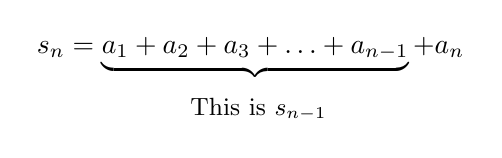
\begin{tikzpicture}
        \node at (0,0) {
          $s_n = \underbrace{a_1+a_2+a_3 + \ldots + a_{n-1}}+ a_n$};
        \node at (.1,-.65) {\small{This is $s_{n-1}$}};
      
      \end{tikzpicture}
  \end{image}

Since $a_n = \frac{n+2}{2n+1}$, we can write

\[
s_n = s_{n-1}+\frac{n+2}{2n+1}.
\] 

Now, if $\lim_{n \to \infty} s_n$ exists and is equal to $L$, we have that $\lim_{n \to \infty} s_{n-1}=L$ as well, so taking the limit of both sides of the above equation gives

\begin{align*}
\lim_{n \to \infty} s_n &= \lim_{n \to \infty} s_{n-1}+ \lim_{n \to \infty} \frac{n+2}{2n+1} \\
L &= L +\frac{1}{2}.
\end{align*} 

This statement is blatantly false, so our underlying assumption that $\lim_{n \to \infty} s_n$ exists is false as well.  Since $\lim_{n \to \infty} s_n$ therefore does not exist,  $\sum_{k=1}^{\infty} \frac{k+2}{2k+1}$ must diverge.
\end{explanation}
\end{example}

As it turns out, the above argument can be used to make a very important observation; if $\{a_n\}$ is a sequence for which $\sum_{k=k_0}^{\infty} a_k$ converges, then $\lim_{n \to \infty} a_n =0$.  This result is fundamentally important, so we capture it in a theorem.

\begin{theorem}
Suppose that $\{a_n\}_{n=n_0}$ is a sequence and the \emph{series} $\sum_{n=n_0}^{\infty} a_n$ converges.  Then, $\lim_{n \to \infty} a_n =0$.   
\end{theorem}

\begin{remark}
Note that the convergence of the \emph{series} $\sum_{n=n_0}^{\infty} a_n$ tells us something about the \emph{sequence} $\{a_n\}$.
\end{remark}

\section{The divergence test}
%The recursive formula does not aid us in finding what the limit of $s_n$ is (and hence does not give the value of $\sum_{k=0}^{\infty} a_k$).  So why would we go to all of the trouble to explore the recursive formula for $s_n$?  As it turns out, it may not tell us much for a convergent series, but let's look at another example.
%
%
%\begin{example}
%Consider the series $\sum_{k=1}^{\infty} \frac{2^k}{k^2+2^k}$.  Note that this is \wordChoice{\choice{a telescoping series}\choice{a geometric series}\choice[correct]{neither a geometric series and it doesn't seem to be a telescoping series}}.  In order to determine whether the series converges, we need to analyze the sequence of partial sums.  
%
%It won't be easy (or maybe even possible) to find an explicit formula for $s_n$, but we can immediately write down a recursive one.
%
%\begin{align*}
%s_n &= s_{n-1}+a_n, \qquad s_1 = a_1 \\
%s_n &= s_{n-1} + \answer[given]{\frac{2^n}{n^2+2^n}}, \qquad s_1 = \answer[given]{\frac{2}{3}}
%\end{align*}
%
%Now, let's assume that $\lim_{n \to \infty} s_n$ exists and $\lim_{n \to \infty} s_n =L$.  Taking limits, we notice something interesting.
%
%\begin{align*}
%\lim_{n \to \infty} s_n &= \lim_{n \to \infty} s_{n-1}+ \lim_{n \to \infty} a_n \\
%\lim_{n \to \infty} s_n &= \lim_{n \to \infty} s_{n-1} +\lim_{n \to \infty} \frac{2^n}{n^2+2^n} \\
%L = L + \answer[given]{1}
%\end{align*}
%where $\lim_{n \to \infty} \frac{2^n}{n^2+2^n}$ is computed using our growth rates results.
%
%This statement gives a contradiction; there is no constant $L$ for which $L=L+1$.  We are thus able to conclude that the assumption that $\lim_{n \to \infty} s_n$ exists is a false one.  This tells us that $\sum_{k=1}^{\infty} \frac{2^k}{k^2+2^k}$ \wordChoice{\choice{converges}\choice[correct]{diverges}} since $\lim_{n \to \infty} s_n$ does not exist.
%\end{example}
%
%As it turns out, the above argument can be used to determine that if $\{a_n\}$ is a sequence whose terms do not tend to zero, the series $\sum_{k=k_0}^{\infty}$ must diverge.  As such, we can write this down as a new criteria.


%As one contemplates the behavior of series, a few facts become clear.
%In order to add an infinite list of nonzero numbers and get a finite
%result, ``most'' of those numbers must be ``very near'' $0$.  Think of 
%this in the opposite sense: what happens if you try to sum $\sum_{n=1}^\infty 2$?
%
%If a series diverges, it means that the sum of an infinite list of
%numbers is not finite (it may approach $\pm \infty$ or it may
%oscillate), and:
%\begin{itemize}
%\item The series will still diverge if the first term is removed.
%\item The series will still diverge if the first $10$ terms are
%  removed.
%\item The series will still diverge if the first $1000000$ terms
%  are removed.
%\item The series will still diverge if \textbf{any finite number} of terms
%  from anywhere in the series are removed.
%\end{itemize}
%
%These concepts are very important and lie at the heart of the next
%theorems.

\begin{theorem}[Divergence test]
 Let $\{a_n\}_{n=n_0}$ be a sequence and consider the series $\sum_{k=k_0}^\infty a_k$.  If $\lim_{n\to\infty}a_n \neq 0$, then $\sum_{n=n_0}^\infty a_n$ diverges.
\end{theorem}

Stated in plain English, the above test ensures that if the terms in a sequence do not tend to zero, then we cannot add all of the terms in that sequence together.

\begin{remark}
The result of this theorem can be established using a similar argument as in the previous example.  Note that there is no explicit reference to the sequence of partial sums in the actual statement of the test.  A more complete statement of the test would be:

\begin{quote}
 Let $\{a_n\}_{n=n_0}$ be a sequence and consider the series $\sum_{k=k_0}^\infty a_k$.  If $\lim_{n\to\infty}a_n \neq 0$, then we can show that $\lim_{n \to \infty} s_n$ does not exist and hence $\sum_{n=n_0}^\infty a_n$ diverges.
\end{quote}

\end{remark}

This test gives us a quick way to determine if some series diverge.

%\begin{example}
%Determine if the series $\sum_{k=1}^{\infty} \frac{2+3k}{1-4k}$ converges or diverges.
%
%\begin{explanation}
%Here, the sequence whose terms are being summed is given by the formula $a_n = \frac{2+3n}{1-4n}$.  Let's try to apply the divergence test.  Notice that the limit of the \emph{sequence} $\{a_n\}$ is $\lim_{n \to \infty} \frac{2+3n}{1-4n} = \answer[given]{-\frac{3}{4}} \neq 0$.  Hence, the \emph{series} $\sum_{k=1}^{\infty} \frac{2+3k}{1-4k}$ diverges by the divergence test.
%
%\end{explanation}
%\end{example}


\begin{example}
Determine if the series $\sum_{k=1}^{\infty} \cos\left(\frac{k^2+7^k}{k!} \right)$ converges or diverges.

\begin{explanation}
Here, the sequence whose terms are being summed is given by the formula $a_n =\cos\left(\frac{n^2+7^n}{n!} \right)$.  Let's try to apply the divergence test.  Notice that

\[
\lim_{n \to \infty} \frac{n^2+7^n}{n!} = \answer[given]{0}
\]
by growth rates, so the limit of the \emph{sequence} $\{a_n\}$ is

\[\lim_{n \to \infty} \cos\left(\frac{n^2+7^n}{n!} \right) = \cos(0) = 1 \neq 0.\]
  
Hence, the \emph{series} $\sum_{k=1}^{\infty} \cos\left(\frac{k^2+7^k}{k!} \right)$ diverges by the divergence test.
\end{explanation}
\end{example}

\begin{example}
Determine if the series $\sum_{k=1}^{\infty} \sin(k)$ converges or diverges.

\begin{explanation}
Here, the sequence whose terms are being summed is given by the formula $a_n =\sin(n)$.  Notice that these terms fluctuate in sign, so maybe when we try adding them all together, we obtain something finite.  Let's try to apply the divergence test.  Notice that $\lim_{n \to \infty} \sin(n)$ does not exist; it certainly is not 0. Hence, the series $\sum_{k=1}^{\infty} \sin(k)$ diverges by the divergence test.
\end{explanation}
\end{example}

\begin{remark}
%While the divergence test provides a quick way to determine that the series in the previous examples diverge, there is valuable intuition that can be gained by taking a step back and thinking about what the limits of the \emph{sequences} whose terms we are trying to sum tells us.  
%
%In the first example, we found $\lim_{n \to \infty} a_n = -\frac{3}{4}$.  This tells us that the terms in the \emph{sequence} we are trying to sum eventually become and stay as close as we want to $-\frac{3}{4}$.  Hence, the infinite \emph{series} $\sum_{k=1}^{\infty} \frac{2+3k}{1-4k}$ requires that we eventually must sum numbers that are arbitrarily close to $-\frac{3}{4}$ indefinitely.  How could this produce a finite result? 

In the last example, perhaps the fact that the terms in $a_n = \sin(n)$ fluctuate in sign will ensure that the series cannot be infinite.  To think about this, let's turn to the sequence of partial sums. To gain a bit of visual perspective about what is happening, note that the $n$-th term in the sequence of partial sums here is 

\[
s_n = \sum_{k=1}^n \sin(k) = \sin(1)+\sin(2)+\ldots+\sin(n).
\]

Plotting several such terms reveals that the terms sequence of partial sums $\{s_n\}$ seem to fluctuate.

\begin{image}
\begin{tikzpicture}
	\begin{axis}[
            domain=.8:6,xmin=0,xmax=16.5,ymin=-.4,ymax=2.5,
            width=4in,
            height=2in,
            axis lines =middle, xlabel=$n$, ylabel=$s_n$,
            xtick={1,2,3,4,5,6,7,8,9,10,11,12,13,14,15,16},
            ytick={1,2},
            every axis y label/.style={at=(current axis.above origin),anchor=south},
            every axis x label/.style={at=(current axis.right of origin),anchor=west},
            clip=false,
            %axis on top,
          ]
       
          \addplot[color=penColor,fill=penColor,only marks,mark=*,ultra thick] coordinates{(1,.84)};  %% closed hole          
          \addplot[color=penColor,fill=penColor,only marks,mark=*,ultra thick] coordinates{(2,1.75)};  %% closed hole 
          \addplot[color=penColor,fill=penColor,only marks,mark=*,ultra thick] coordinates{(3,1.89)};  %% closed hole  
          \addplot[color=penColor,fill=penColor,only marks,mark=*,ultra thick] coordinates{(4,1.14)};  %% closed hole
           \addplot[color=penColor,fill=penColor,only marks,mark=*,ultra thick] coordinates{(5,.18)};  %% closed hole
           \addplot[color=penColor,fill=penColor,only marks,mark=*,ultra thick] coordinates{(6,-.1)};  %% closed hole
           \addplot[color=penColor,fill=penColor,only marks,mark=*,ultra thick] coordinates{(7,.55)};  %% closed hole
           \addplot[color=penColor,fill=penColor,only marks,mark=*,ultra thick] coordinates{(8,1.54)};  %% closed hole
           \addplot[color=penColor,fill=penColor,only marks,mark=*,ultra thick] coordinates{(9,1.96)};  %% closed hole
           \addplot[color=penColor,fill=penColor,only marks,mark=*,ultra thick] coordinates{(10,1.41)};  %% closed hole
           \addplot[color=penColor,fill=penColor,only marks,mark=*,ultra thick] coordinates{(11,.41)};  %% closed hole
           \addplot[color=penColor,fill=penColor,only marks,mark=*,ultra thick] coordinates{(12,-.13)};  %% closed hole
           \addplot[color=penColor,fill=penColor,only marks,mark=*,ultra thick] coordinates{(13,.29)};  %% closed hole
           \addplot[color=penColor,fill=penColor,only marks,mark=*,ultra thick] coordinates{(14,1.29)};  %% closed hole
           \addplot[color=penColor,fill=penColor,only marks,mark=*,ultra thick] coordinates{(15,1.94)};  %% closed hole
           \addplot[color=penColor,fill=penColor,only marks,mark=*,ultra thick] coordinates{(16,1.65)};  %% closed hole  
        \end{axis}
\end{tikzpicture}
\end{image}

While we will not show it here, the sequence $\{s_n\}$ is bounded; the reason that $\lim_{n \to \infty} s_n$ does not exist is due to the fact that the terms fluctuate (meaning that the sequence is never eventually monotonic). 
\end{remark}



%\begin{warning}
%Notice that the divergence test allows us to determine that the \emph{series} $\sum_{k=1}^{\infty} a_k$ diverges in the above examples by analyzing the limit of the \emph{sequence} $\{a_n\}$.  The divergence test is an actual theorem; it is a result that allows us to use information about $\lim_{n \to \infty} a_n$ to determine if $\sum_{k=1}^{\infty}$ diverges rather than having to analyze $\lim_{n \to \infty} s_n$ explicitly.  While it may be difficult to digest, it is important to understand the logic behind this  \textbf{<---Jim: I can't think of exactly what I want to say here...something along the lines of emphasizing they must be aware of what notation is, what concepts the notation represents, etc...let's discuss}
%\end{warning}

\section{Implications of the divergence test}

Let's summarize the important points from the previous discussion.

\begin{itemize}
\item If $\sum_{k=k_0}^\infty a_k$ converges, then $\lim_{n \to \infty} a_n =0$.
\item If $\lim_{n \to \infty} a_n \neq 0$ (including the case where the limit does not exist), then $\sum_{k=k_0}^{\infty} a_k$ diverges.
\end{itemize}

%\textbf{Jim: do we use the word contrapositive here and explain to those unfamiliar with it why one statement follows from each other?} 

While divergence test was straightforward to apply in the previous examples, there is a major point to address about what it does \emph{not} say.

\begin{quote}
  The divergence test can \emph{never} be used to conclude that a series converges. The theorem \emph{does not state} that if $\lim_{n\to\infty} a_n =
  0$ then $\sum_{n=1}^\infty a_n$ converges.

\end{quote}
  
%\begin{warning}
%  The divergence test can \emph{never} be used to conclude that a series converges.  The theorem \emph{does not state} that if $\lim_{n\to\infty} a_n =
%  0$ then $\sum_{n=1}^\infty a_n$ converges.
%\end{warning}

We've actually seen an example of this in action.  

\begin{example}
Recall that in a previous section, we showed that the series $\sum_{k=1}^\infty \ln\left(\frac{k+1}{k}\right)$ is actually telescoping.  By recognizing that $\ln\left(\frac{k+1}{k}\right) = \ln(k+1)-\ln(k)$, we showed that there is an explicit formula for the $n$-th term in the sequence of partial sums given by $s_n = \ln(n+1)$.  We concluded that $\sum_{k=1}^\infty \ln\left(\frac{k+1}{k}\right)$ diverges since $\lim_{n \to \infty} s_n = \infty$.   

Note now that the expression in the sum (i.e. the sequence whose terms we are attempting to sum) is $a_n =   \ln\left(\frac{n+1}{n}\right)$, and that since

\[
\lim_{n \to \infty} \frac{n+1}{n} = \answer[given]{1}
\]
we have

\[
\lim_{n \to \infty} \ln\left(\frac{n+1}{n}\right) = \ln\left(\answer[given]{1}\right) = 0.
\]

Thus, we have an example of a \emph{sequence} whose limit is zero for which the sum of its terms diverges; that is, we have an example where $\lim_{n \to \infty} a_n =0$ but $\sum_{k=1}^{\infty} a_k$ diverges.
\end{example}


\begin{remark}
The standard example of a sequence for which $\lim_{n \to \infty} a_n =0$ but for which $\sum_{k=1}^{\infty} a_k$ diverges is the harmonic series, $\sum_{k=1}^{\infty} \frac{1}{k}$.  We'll show later on that this series diverges.
\end{remark}

Said another way: 
\begin{quote}
If $\sum_{k=k_0}^{\infty} a_k$ diverges, it's still possible that  $\lim_{n \to \infty} a_n =0$. 
\end{quote}
  
\begin{question}
To elaborate a little more, we can say that a series $\sum_{k=k_0} a_k$ ``passes the divergence test'' if $\lim_{n \to \infty} a_n=0$.  Which of the following series pass the divergence test?
\begin{selectAll}
	\choice[correct]{$\sum_{k=3}^\infty \frac{1}{\ln{ k }}$}
	\choice{$\sum_{k=0}^\infty \sin(k)$}
	\choice[correct]{$\sum_{k=0}^\infty \frac{\sin(k)}{k^2}$}
	\choice{$\sum_{k=5}^\infty \frac{k+7}{k+6}$}
	\choice{$\sum_{k=0}^\infty \frac{2k}{k - 5}$}
\end{selectAll}
\end{question}

Restating this point again (because it is very important): passing the divergence test 
means that a series has a chance to converge.  The divergence test cannot tell us 
whether a series converges.

%\begin{question}
%Which of the following statements are true?  Mark all that apply.
%\begin{selectAll}
%  \choice[correct]{If $\sum_{k=0}^\infty a_k$ is convergent, then $\lim_{k \to \infty} a_k = 0$. }
%  \choice{If $a_k \to 0$ as $k \to \infty$, then $\sum_{k=0}^\infty a_k$ is convergent.}
%  \choice{If $\sum_{k=0}^\infty a_k$ is divergent, then $\lim_{k \to \infty} a_k \neq 0$. }
%  \choice[correct]{If $\lim_{k \to \infty} a_k \neq 0$, then $\sum_{k=0}^\infty a_k$ is divergent.}
%\end{selectAll}
%\end{question}
%
%
%\section{Conceptual questions}
There are many questions that require that you now have a firm grasp on the concepts presented thus far.  We summarize the important points made thus far, then give many examples that require you to synthesize them.

\begin{itemize}
\item There are two fundamental questions we can ask of \emph{any} sequence.
\begin{itemize}
\item[1.] Do the numbers in the list approach a finite value?
\item[2.] Can I sum all of the numbers in the list and obtain a finite result?
\end{itemize}
These questions can be asked of a given sequence $\{a_n\}$ and can also be asked about $\{s_n\}$ or any sequence constructed from it.
\item Given a sequence $\{a_n\}_{n=n_0}$, we construct the sequence of partial sum $\{s_n\}_{n=n_0}$ whose $n$-th term is given by the formula $s_n = \sum_{k=k_0}^n a_k$.
\begin{itemize}
\item The symbols $\sum_{k=k_0}^{\infty} a_k$ and $\lim_{n \to \infty} s_n$ are the same.
\item By definition $\sum_{k=k_0} a_k$ converges if $\lim_{n \to \infty} s_n$ exists and in this case, the value of each is the same.
\item By definition $\sum_{k=k_0} a_k$ diverges if $\lim_{n \to \infty} s_n$ does not exist (which includes if the limit is infinte). 
\end{itemize}
\item If the limit of a \emph{sequence} is not zero, the sum of its terms diverges.
\item If a series converges, the limit of the sequence whose terms is being summed is zero.
\item If the limit of a sequence is zero, more information is needed to determine whether the sum of its terms converges or diverges.
\end{itemize}

To answer the following questions, make sure that you understand exactly what is given in the statement of the question first, then try to synthesize the material above.

\begin{example}
Suppose that $\{a_n\}_{n=1}$ is a sequence and let $s_n = \sum_{k=1}^{n} a_k$.  Suppose that it is also known that $s_n = \frac{2n+6}{n+4}$.

\begin{question}
Which statement below captures the most we can say about $\sum_{k=1}^{\infty} a_k$? 

\begin{multipleChoice}
\choice{$\sum_{k=1}^{\infty} a_k$ converges but we cannot determine its value without more information.}
\choice{$\sum_{k=1}^{\infty} a_k$ converges to $0$.}
\choice[correct]{$\sum_{k=1}^{\infty} a_k$ converges to $2$.}
\choice{$\sum_{k=1}^{\infty} a_k$ diverges.}
\choice{More information is needed to determine if $\sum_{k=1}^{\infty} a_k$ converges.}
\end{multipleChoice}

\begin{feedback}
The information given in the problem is an explicit formula for the terms in the \emph{sequence of partial sums} $s_n$, not $a_n$.  To answer this question, we need to know how $s_n$ relates to finding $\sum_{k=1}^{\infty} a_k$.  Since $\lim_{n \to \infty} s_n$ and $\sum_{k=1}^{\infty}$ are analogous representations of the same idea and $\lim_{n \to \infty} s_n = \answer[given]{2}$, we have $\sum_{k=1}^{\infty} a_k$ converges to $2$. 
\end{feedback}
\end{question}
%%%%%%%%%%%%%%%%%
\begin{question}
Which statement below captures the most we can say about $\sum_{k=1}^{\infty} s_k$? 

\begin{multipleChoice}
\choice{$\sum_{k=1}^{\infty} s_k$ converges but we cannot determine its value without more information.}
\choice{$\sum_{k=1}^{\infty} s_k$ converges to $0$.}
\choice{$\sum_{k=1}^{\infty} s_k$ converges to $2$.}
\choice[correct]{$\sum_{k=1}^{\infty} s_k$ diverges.}
\choice{More information is needed to determine if $\sum_{k=1}^{\infty} s_k$ converges.}
\end{multipleChoice}

\begin{feedback}
It may seem daunting to think about what $\sum_{k=1}^{\infty} s_k$ is in general, but note here that the information given in the problem is an explicit formula for $s_n$.  $\{s_n\}_{n=1}$ is a sequence in its own right, and we can ask whether we can sum its terms.  Here, we can immediately write down the series in question.

\[
\sum_{k=1}^{\infty} s_k =\sum_{k=1}^{\infty} \frac{2k+6}{k+4}
\]
Since $\lim_{n \to \infty} s_n = 2\neq 0$, we have $\sum_{k=1}^{\infty} s_k$ diverges by the divergence test. 
\end{feedback}
\end{question}

Note that in the previous questions, $\lim_{n \to \infty} s_n$ was used in two different ways.  For the first question, $\lim_{n \to \infty} s_n$ is used to answer a question about $\sum_{k=1}^{\infty} a_k$ by using the definition of convergence.  In the second question, we are asked to think of $\{s_n\}$ as a sequence in its own right whose terms can be summed.  We can use the divergence test to answer this question.
\end{example}

\begin{example}
Suppose that $\{a_n\}_{n=1}$ is a sequence and let $s_n = \sum_{k=1}^{\infty} a_k$.  Suppose that it is known that $\sum_{k=1}^{\infty} s_k =3$.  What can be said about $\sum_{k=1}^{\infty} a_k$?

\begin{multipleChoice}
\choice{$\sum_{k=1}^{\infty} a_k$ converges but we cannot determine its value without more information.}
\choice[correct]{$\sum_{k=1}^{\infty} a_k$ converges to $0$.}
\choice{$\sum_{k=1}^{\infty} a_k$ converges to $3$.}
\choice{$\sum_{k=1}^{\infty} a_k$ diverges.}
\choice{More information is needed to determine if $\sum_{k=1}^{\infty} a_k$ converges.}
\end{multipleChoice}

\begin{feedback}
The information given in the problem is that $\sum_{k=1}^{\infty} s_k$ is a convergent series.  We need to relate this to $\sum_{k=1}^{\infty} a_k$.  The relationship between the sequence of partial sums and $\sum_{k=1}^{\infty} a_k$ is that $\lim_{n \to \infty} s_n$ and $\sum_{k=1}^{\infty} a_k$ are analogous, so we need $\lim_{n \to \infty} s_n$.  Thankfully, we have a fact for that; since $\sum_{k=1}^{\infty} s_k$ is convergent, the limit of the inner sequence whose terms we add must be zero; that is  $\lim_{n \to \infty} s_n=0$.  Hence, $\sum_{k=1}^{\infty} a_k=0$.
\end{feedback}

\end{example}

\begin{question}
  Suppose $\{a_n\}_{n \geq 1}$ is a sequence and $\sum^{\infty}_{n= 1}
  a_n=5$.  Let $s_n = \sum^n_{k=1} a_k$. Select all
  statements that must be true:
  \begin{selectAll}
    \choice{$\lim_{n \to \infty} a_n = 5$}
    \choice[correct]{$\lim_{n \to \infty} a_n = 0$}
    \choice{$\lim_{n \to \infty} s_n = 0$}
    \choice[correct]{$\lim_{n \to \infty} s_n = 5$}
    \choice[correct]{$\sum^{\infty}_{k=1} s_k$ must diverge.}
    \choice{$\sum^{\infty}_{k=1} (a_k+1) = 5+1=6$}
    \choice{The divergence test tells us $\sum^{\infty}_{n= 1} a_n$ converges to $L$.}
  \end{selectAll}
  
\begin{feedback}
Let's look at each of these statements.
\begin{itemize}
\item For the first four choices, notice that since $\sum_{k=1}^{\infty} a_k =5$, we have two immediate consequences.  First, by definition $\lim_{n \to \infty} s_n = 5$.  Secondly, $\sum_{k=1}^{\infty} a_k$ converges, so $\lim_{n \to \infty} a_n = 0$.
\item Now that we know $\{s_n\}$ is a sequence that does not tend to zero, the divergence test tells us we cannot sum its terms; i.e. since $\lim_{n \to \infty} s_n \neq 0$, $\sum_{k=1}^{\infty}$ must diverge.
\item First, notice that there is a huge difference in the series $\sum^{\infty}_{n=1} (a_n+1)$ and $\sum^{\infty}_{n=1} a_n+1$, where the latter sum is to be interpreted as $\left(\sum^{\infty}_{n=1} a_n\right)+1$.  Since $\lim_{n \to \infty} a_n =0, \lim_{n \to \infty} (a_n+1) \neq 0$, so $\sum^{\infty}_{k=1} (a_k+1)$ diverges by divergence test.
\item The last choice is never true; we can \emph{never} determine that a series converges by the divergence test.
 \end{itemize}
\end{feedback}
  
\end{question}

%\begin{question}
%  Suppose that $\seq{a_n}_{n \geq 1}$ is a \emph{decreasing} sequence.
%  Let $S_n = \sum^n_{k=1} a_k$ and suppose $\lim_{n \to \infty} S_n$
%  does not exist. Select all statements that must be true:
%  \begin{selectAll}
%    \choice{$\lim_{n \to \infty} a_n$ does not exist.}
%    \choice{$\sum^{\infty}_{k=1} a_k$ could converge.}
%    \choice[correct]{$\sum^{\infty}_{n=1} S_n$ must diverge.} 
%    \choice{$\seq{S_n}$ must be monotonic.}
%    \choice{$\seq{S_n}$ must be bounded.}
%    \choice{$\lim_{n \to \infty} S_n = -\infty$}
%    \choice{The divergence test applied to $\sum^{\infty}_{k= 1} a_k$ would
%      guarantee that $\sum^{\infty}_{k=1} a_k$ diverges.}
%  \end{selectAll}
%\end{question}
%
%
%\begin{question}
%  Suppose that $\seq{a_n}_{n \geq 1}$ is a sequence with $a_n > 0$ for all $n \geq 1$.
%  Let $S_n = \sum^n_{k=1} a_k$ and suppose $\lim_{n \to \infty} S_n =
%  L$. Select all statements that must be true:
%  \begin{selectAll}
%    \choice[correct]{$\sum^{\infty}_{k=1} a_k = L$}
%    \choice[correct]{$\lim_{n \to \infty} a_n = 0$}
%    \choice[correct]{$\seq{S_n}$ must be monotonic}
%    \choice[correct]{$\seq{S_n}$ must be bounded}
%    \choice{$\sum^{\infty}_{n=1} (a_n-L) = 0$}
%    \choice[correct]{$\sum^{\infty}_{n=1} S_n$ must diverge}
%    \choice{The divergence test applied to $\sum^{\infty}_{k= 1} a_k$ would
%      guarantee that $\sum^{\infty}_{k=1} a_k$ converges.}
%  \end{selectAll}
%\end{question}
%
%It's a great idea at this point to stop and compare the previous two questions.









\end{document}


